\chapter{Implementation and code generation}
\label{chapter:process:implementation}

Folderol\footnote{\url{https://github.com/amosr/folderol}} is a Haskell implementation of Machine Fusion \REFTODO{fusion}.
Machine Fusion uses the topology of the entire process network to perform fusion.
When fusing one producer with multiple consumers, the fusion algorithm must coordinate between all the consumers to reach consensus on when to pull the next value.
This coordination between all consumers means the fusion algorithm requires global knowledge of the process network.
In contrast, shortcut fusion systems \REFTODO{shortcut} use rewrite rules to remove intermediate buffers and require only local knowledge, but cannot coordinate between multiple consumers.
In cases where shortcut fusion cannot fuse it fails silently, leaving the programmer unaware of the failure.
This silence is also due to the local nature of rewrite rules: if we wish to know whether all the processes have been fused, we need to know about all the processes.
To fuse the entire process network, as well as to inform the programmer when fusion fails, Folderol uses Template Haskell, a form of metaprogramming.

This chapter looks at the implementation of Folderol, in particular how to generate efficient code for a fused process.
Generating code for a single process is fairly straightforward in itself: the process language is a simple imperative language, and once the process network has been fused into a single process there is no longer any need for threading or inter-process communication.
However, code generation needs to be tailored specifically to take advantage of the optimisations in the target compiler, which in this case is the Glasgow Haskell Compiler (GHC).
Haskell does support imperative constructs like mutable references, but being a functional language, the optimisations in GHC are more geared towards functional programs.
Mutable references are not optimised particularly well.
If we wish to generate efficient code, we must --- perhaps surprisingly --- avoid mutable references, and generate code closer to what the compiler expects.

\section{Template Haskell}
Template Haskell is a metaprogramming extension for Haskell \cite{sheard2002template} which provides a limited form of staged computation, where the only `stages' are compile-time and runtime.
There are two variants of Template Haskell: untyped and typed.
Untyped Template Haskell does not enforce well-typedness of the generated program until after the program is generated, which means it is quite easy to generate ill-typed programs.
Even though we can generate ill-typed programs, overall soundness is preserved because the generated program is still typechecked and compiled at compile-time.
On the other hand, typed Template Haskell enforces well-typedness of the generated program by lifting types in the generated program up to the meta-level as types in the generator program.

We use untyped Template Haskell for code generation.
Performing typed code generation is equivalent to proving that the result program is well-typed, whereas untyped code generation requires no such proof.
This makes the untyped version easier to implement.
While typed code generation is no doubt possible, it is an interesting research problem on its own \CITE{Accelerate}.

The problem with using untyped code generation is that if there are type errors they will not be found until quite late, once the generated code has been spliced into the main program.
This means that when the programmer sees the type error, the error location will be in the generated code.
That is, the error is shown in code the program wrote, rather than code the programmer wrote.
This complicates finding the underlying cause of the error and fixing the problem.
Type safety is a big problem when we wish to provide a library for other programmers: it is unacceptable to require a user of the library to understand the internal workings of code generation to understand type errors.
Typed Template Haskell allows us to provide a type-safe interface to users of the library.

\subsection{Untyped expressions}
\TODO{find a better example. This is placeholder.}

Template Haskell extends regular Haskell with two syntactic constructs: quasiquoting and splicing, for moving between runtime and compile-time stages.
Quasiquoting converts a runtime expression to a compile-time value, while splicing performs the opposite conversion.
For example, we can quasiquote some arithmetic using the syntax \lstinline/[|1+2|]/, which produces the corresponding abstract syntax tree for an infix operator with two integer arguments:

\begin{lstlisting}
InfixE (Just (LitE (IntegerL 1))) (VarE GHC.Num.+) (Just (LitE (IntegerL 2)))
\end{lstlisting}

Quasiquoting is a purely syntactic convenience, as any quasiquoted expressions could be produced using the abstract syntax tree constructors directly.
That said, it is a particularly useful convenience which we will use extensively.

Splicing takes a compile-time abstract syntax tree and converts it to an expression to be evaluated at runtime.
For example, splicing back the quasiquoted arithmetic using the syntax \lstinline/$([|1+2|])/, will evaluate (@1+2@) at runtime.

Splicing and quasiquoting operate in the @Q@ monad.
The @Q@ monad gives a fresh name supply, so that when names are bound inside expressions they can be given unique names.
These fresh names ensure that newly bound names will not interfere with existing bindings.

Now let us look at a concrete example of how to use Template Haskell.
Suppose we wish to define a power function where the exponent is known at compile time, but the mantissa is not known until runtime.

We define @power@ as a function with the type \lstinline/Int ->  Q Exp/.
This means it takes an integer at compile-time, and produces a quoted expression in the quote monad.
This result expression will, once spliced in, have type \lstinline/Int ->  Int/.
Later we shall use typed Template Haskell to make this extra type information explicit, but for now we must perform typechecking in our heads.

\begin{lstlisting}
power :: Int -> Q Exp
power 0 = [|\m -> 1                      |]
power e = [|\m -> $(power (e - 1)) m * m |]
\end{lstlisting}

The @power@ function pattern-matches on the exponent.
When the exponent is zero, we enter quasiquoting mode and construct a function that always returns one.
When the exponent is non-zero, we again enter quasiquoting mode and construct a function, taking the mantissa as its argument.
Inside the quasiquote, we need to handle the recursive case for the one-smaller exponent (\lstinline/e - 1/), so we enter into splicing mode with \lstinline/$(power (e - 1))/ to compute the one-smaller power.
The splice for the one-smaller power returns a function, to which we apply the mantissa.
Finally, we multiply the one-smaller power of the mantissa by the mantissa itself.

We can now define a specialised @power@ function to compute the square.
We define this as a top-level binding which performs a splice, and inside that splice we call @power@ with the statically known argument @2@.
The type inside the splice is \lstinline/Q Exp/, and once splicing is complete the result is an expression of type \lstinline/Int ->  Int/.

\begin{lstlisting}
power2 :: Int -> Int
power2 = $(power 2)
\end{lstlisting}

The reason for this specialisation is to produce optimised code: by knowing the exponent at compile-time, we can perform the recursion once at compile-time rather than many times at runtime.
It is therefore worth inspecting the resulting code to check whether it is indeed optimal.
The compiler option (@-ddump-splices@) outputs the result splices, as follows.

\begin{lstlisting}
$(power 2) =
  \m0 -> (\m1 -> (\m2 -> 1) m1 * m1) m0 * m0
\end{lstlisting}

This is a roundabout way to multiply a number by itself, and there are a lot of opportunities to simplify that code.
While we expect the compiler to remove the extra lambdas by beta reduction, it would be even better to not introduce them in the first place.
If we do not introduce simplification opportunities in the first case, there is no uncertainty about whether the compiler will be able to remove them.
The problem is that @power@ introduces a lambda for each recursive step, while we only want one lambda at the top-level.
So let us fix this by defining a top-level function which introduces the lambda, and a recursive helper function to compute the power.

\begin{lstlisting}
powerS :: Int -> Q Exp
powerS e = [|\m -> $(powerS' e [|m|])|]
\end{lstlisting}

The top-level function @powerS@ introduces the lambda for the mantissa inside a quasiquote, then calls the helper function @powerS'@.
The exponent is a compile-time binding, while the mantissa is a runtime binding.
When the helper function is called at compile-time, the exponent can be passed as-is, while the mantissa must be quasiquoted to wrap the runtime binding into a compile-time expression.

The recursive helper function, @powerS'@, has type \lstinline/Int ->  Q Exp ->  Q Exp/.

\begin{lstlisting}
powerS' :: Int -> Q Exp -> Q Exp
powerS' 0 m = [|1                        |]
powerS' e m = [|$(powerS' (e-1) m) * $(m)|]
\end{lstlisting}

Like the original @power@ function, it pattern-matches on the exponent and in the recursive case multiplies by itself.
The difference is that the mantissa is bound as a compile-time expression with type (@Q Exp@) rather than inside the quasiquote, so it must be spliced when it is used.

The output for (@powerS 2@) is a lot simpler than that for (@power 2@).
Whereas before there was a lambda introduced and applied at each recursive step, now there is only a single lambda.

\begin{lstlisting}
$(powerS 2) =
  \m -> ((1 * m) * m)
\end{lstlisting}

There is still more we could do to improve the function: for example, (@1 * m@) could be replaced by @m@.
However, this is sufficient to show the core splicing and quoting ideas behind Template Haskell.
For more information on staging in general, \citet{rompf2010lightweight} takes this example further.

\subsection{Typed expressions}

% The problem with Template Haskell shown above is that there are no types attached to expressions.
% Quasiquoting a string \lstinline/[|"one"|]/ and quasiquoting an integer \lstinline/[|1|]/ both produce a value of the same type: @Q Exp@.
% We can then use these expressions to construct larger, completely untypable expressions; for example we could try to subtract a string from an integer, which should surely fail: \lstinline/[|1 - "one"|]/.

Typed Template Haskell extends the Template Haskell we have seen with typed expressions, typed splicing and typed quasiquoting.
The type of typed expressions, @TExp@, is annotated with a meta-level (compile-time) type argument denoting the object-level type of the expression.
Syntactically, typed quasiquotation uses two pipes, while typed splicing uses two dollar signs.
For example, using a typed quasiquote on a string will produce a @String@-typed expression: (\lstinline/[||"one"||] :: Q (TExp String)/).
Similarly, typed splicing eliminates the @Q@ monad and the @TExp@ wrapper, leaving only the result type: (\lstinline/$$([||"one"||]) :: String/).

Typed expressions are invaluable for providing a typesafe way to construct process networks.
We need to construct process networks at compile-time to fuse them at compile-time, while keeping the information required to execute them at runtime.
Consider the standard @filter@ function for lists, with type (\lstinline/(a ->  Bool) ->  [a] ->  [a]/).
In order to implement a process network version of @filter@, the function argument of type (\lstinline/(a ->  Bool/) must be converted to an expression, as it will be evaluated and applied at runtime.
Providing a process network @filter@ function which takes as an argument the typed expression (\lstinline/Q (TExp (a ->  Bool))/) instead of the untyped expression (\lstinline/Q Exp/) means that type errors can be caught early.

We provide an untyped core for the processes and networks, then build on top of this to provide a typed interface for constructing networks.
For this reason, we need to be able to convert from typed expressions to untyped expressions.
We can convert from a typed expression to an untyped expression using the @unTypeQ@ function, which has type (\lstinline/Q (TExp a) ->  Q Exp/).
This does not affect the underlying expression, it just throws away the meta-level type information.
The object-level type information remains, and once it is spliced in it will have the same type.

% Conversely, if one is very careful, one can convert an untyped expression to a typed one.
% This is an unsafe operation, because one can choose any type at all for the expression.
% The expression is not checked against the chosen type until it is spliced in.
% \begin{lstlisting}
% unsafeTExpCoerce :: Q Exp -> Q (TExp a)
% \end{lstlisting}
 
% By using untyped expressions for code generation, we do not lose any actual type safety, since the generated code will still end up being typechecked by the Haskell compiler.
% What we do lose are good error locations, but these errors will only occur if there are bugs in the code generator.
% Any type errors in the user of the library will be using the typesafe interface, with better error messages.

% Although it is possible to construct expressions with the wrong type, this generally requires explicitly unsafe operations.
% Most of the time, this is unlikely to occur by accident alone.

\section{Constructing a process network}
\label{s:extraction:grepGood}

The following example constructs a process network in Folderol.
In due course we will inspect its generated code, but first it is necessary to see how process networks are constructed.

\begin{lstlisting}
grepGood :: FilePath -> FilePath -> IO ()
grepGood fileIn fileOut =
  $$(fuse $ do
     input  <- source [||sourceOfFile fileIn ||]
     goods  <- filter [||isPrefixOf   "Good" ||] input
     sink      goods  [||sinkToFile   fileOut||])
\end{lstlisting}

This example reads input lines from a file, filters out all except those starting with the string \lstinline/"Good"/, and finally writes the results to file.
In a Unix-style environment, we would write this as ``@grep ^Good@''; the caret (@^@) meaning ``starting with''.

The function @grepGood@ takes two arguments of type @FilePath@ for the input and output filenames.
Inside the definition, the Template Haskell splice \lstinline/$$(fuse ...)/ takes the process network as an argument, fuses the processes together, and generates output code.
We are constructing the process network inside the Template Haskell splice at compile-time, while we wish to execute it at runtime.
The process network is the static representation of the computation, and must be statically known and finite.

Inside the process network we start by creating a \emph{source} to read from the input file @fileIn@.
The @source@ function creates an input stream in the process network which can be used by other processes.
The @input@ binding in this case refers to the abstract name of the stream in the process network, rather than the runtime values of the stream.
This is an important distinction, as expressions operating over runtime values need to be quasiquoted to delay them from compile-time to runtime.
Similarly, the input file @fileIn@ will not be known until runtime.
The choice of source does not affect fusion, and does not need to be known at compile time.
Since most sources depend on runtime values in some way, the entire source is delayed until runtime and must be quasiquoted.

Now we take the values in the @input@ stream and filter them to those starting with the string \lstinline/"Good"/.
Again considering the compile-time/runtime distinction, the fact that the @filter@ process uses the stream named @input@ as its input is known at compile-time, and is not quasiquoted; while the predicate, which depends on the runtime stream values, must be quasiquoted.
We call the output filtered stream @goods@.

Finally, we send the filtered output to a file, by creating a \emph{sink}.
The @sink@ function is the opposite of @source@, and just like @source@ it requires the description of how to sink (writing to a file using @sinkToFile@) to be quasiquoted.

\TODO{Show the process network and the processes.}
Soon enough, we shall return to this.


% \begin{lstlisting}
% applyTransactions :: FilePath -> FilePath -> IO ()
% applyTransactions fileIn fileOut =
%   $$(fuse $ do
%      cust  <- source [||sourceOfFile fileCust||]
%      txns  <- source [||sourceOfFile fileTxns||]
%      cust' <- map    [||parseCust            ||] cust
%      txns' <- map    [||parseTxns            ||] txns
% 
%      (newCust, invalid) <- groupLeft [||applyTxn||] cust' txns'
% 
%      sink newCust [||sinkToFile fileOutCust   ||]
%      sink invalid [||sinkToFile fileOutInvalid||])
% \end{lstlisting}

% We start with the Template Haskell splice \lstinline/$$(fuse ...)/. In the code it is blue. 
% It has the following type.
% \begin{lstlisting}
% fuse :: Network () -> Q (TExp (IO ()))
% \end{lstlisting}
% That is, it takes a process network and returns the expression for the underlying @IO@ computation.
% The process network @Network ()@ is a monad as well.
% 
% The process network first constructs a source that reads from a file.
% \begin{lstlisting}
% source :: Q (TExp (Source a))                -> Network (Channel a)
% filter :: Q (TExp (a -> Bool))  -> Channel a -> Network (Channel a)
% map    :: Q (TExp (a -> b))     -> Channel a -> Network (Channel b)
% sink   :: Q (TExp (Sink a))     -> Channel a -> Network (Channel a)
% \end{lstlisting}
% The @source@ function takes a quasiquoted expression of how to construct the source at runtime.
% 
% Now show the generated code.
% 



\section{All this boxing and unboxing}
\TODO{Reorganise: what does boxing have to do with fusion?}

In Haskell, most values are boxed by default \citep{jones1991unboxed}.
Boxed values are stored as pointers to heap objects, which can in turn reference other boxed or unboxed values.
Pointers have a uniform representation regardless of the type of the object they point to.
This uniform representation allows the same generated code for a polymorphic data structure or function to be used for any boxed type.
A list which is polymorphic in its element type can use the same pointer type to refer to its values regardless of the actual element type.

The problem with boxed values is that they require at least one allocation per object and a pointer indirection for each access.
Incrementing an unboxed integer stored in a register is a single instruction.
Incrementing a boxed integer requires more work.
First the value is read from memory into a register, where it is incremented.
In Haskell most heap objects are immutable; rather than updating the original heap object, a new object must be allocated.
Finally, the newly allocated object is filled in by copying the value from the register to memory.
This copying and allocation makes boxed arithmetic at least an order of magnitude slower than unboxed arithmetic.

Consider the following function, which loops over an array to compute its sum.
The function starts by calling the local function @loop@ with the initial loop index, and the initial sum.
The definition of @loop@ checks if it has reached the end of the array, and if so returns the sum; otherwise it increments the running sum and proceeds to the next index.

\begin{lstlisting}
sum :: Vector Int -> Int
sum vector = loop 0 0
 where
  loop index running_sum
   | index == length vector
   = running_sum
   | otherwise
   = let value = vector ! index
     in loop (index + 1) (running_sum + value)
\end{lstlisting}

Inside the loop, the loop index and the running sum are both boxed values because their type (@Int@) is boxed; this is not explicit in the program source.
This function, if compiled naively, would spend more time boxing and unboxing than actually computing the sum.
For each element of the array, the function allocates two new boxed values: the updated index and the updated sum.
All of these new boxed values except the very last iteration are used once by the next iteration and then thrown away.
While the garbage collector is tuned for small, short-lived objects, it is better to not create any garbage in the first place.

Compiler optimisations to replace boxed values with unboxed values are well-known, and there are many different ways to do this.
\TODO{More concrete.}
The point to make is not that this is an interesting thing, just that we must know which optimisations our compiler performs to generate code that our compiler can optimise.

In GHC, boxed machine-word integers are represented by the following type, which defines @Int@ with a single constructor @I#@, taking an unboxed integer @Int#@. By convention, unboxed values and constructors that use them are named with the @#@ suffix.

\begin{lstlisting}
data Int = I# Int#
\end{lstlisting}

Now we know how machine-word integers are represented, we can look at an explicitly boxed version of @sum@.
This version still uses boxed integers, but all arithmetic operations explicitly unbox and rebox the arguments and return values.
Unboxed literals are written as @0#@ or @1#@.
Unboxed arithmetic operations are written as @+#@ or @==#@, and @!#@ for unboxed indexing.
With explicit boxing, it should now be visible that the recursive call to @loop@ constructs new boxed integers.

\begin{lstlisting}
sum :: Vector Int -> Int
sum vector = loop (I# 0#) (I# 0#)
 where
  loop (I# index) (I# running_sum)
   | index ==# length vector
   = I# running_sum
   | otherwise
   = let value = vector !# index
     in loop (I# (index +# 1#)) (I# (running_sum +# value))
\end{lstlisting}

Constructor specialisation \cite{peyton2007call} is a loop optimisation that can remove these boxed arguments to recursive calls.
Constructor specialisation starts by looking at the constructor arguments to recursive calls, and notes which ones are scrutinised or unwrapped at the start of the function definition.
In the explicitly boxed @sum@ function, @loop@ is first called with the constructors @I#@ for both arguments, and both of these arguments are scrutinised by @loop@.
Based on this information, constructor specialisation creates a specialised version of @loop@ to be used when both arguments are @I#@ constructors.
This specialised version is based on the original, except each argument of a known constructor is replaced by the constructor's arguments, and pattern matches on a known constructor are simplified away.
We call this specialised version @loop'I#'I#@.
Everywhere that @loop@ is called with @I#@ constructors, it is replaced by a call to the specialised function @loop'I#'I#@.
For example, the initial call (@loop (I# 0#) (I# 0#)@) is replaced by (@loop'I#'I# 0# 0#@).

\begin{lstlisting}
sum :: Vector Int -> Int
sum vector = loop'I#'I# 0# 0#
 where
  loop'I#'I# index running_sum
   | index ==# length vector
   = I# running_sum
   | otherwise
   = let value = vector !# index
     in loop'I#'I# (index +# 1#) (running_sum +# value)
\end{lstlisting}

Constructor specialisation has removed all the boxing except for the final return value, which is only constructed once anyway.
The original @loop@ function was no longer called, so it was able to be removed entirely.
The original function cannot always be removed, and constructor specialisation can create many specialisations: one for each combination of constructors.
When there are a lot of combinations, the computer might not have enough memory to store every specialised function at the same time.
To alleviate this, GHC implements some heuristics to limit the number of specialisations, as well as only creating specialisations if the original function is not too large.
This makes sense for general purpose code, but for tight loops where we expect most of our runtime to be, we need to be sure that all specialisations are created.
For tight loops, we want to \emph{force} constructor specialisation to specialise everything.
We force constructor specialisation by annotating the function to be specialised with an extra argument of the special constructor @SPEC@.
Going back to the original version of the @sum@ function, we force constructor specialisation on @loop@ by adding the @SPEC@ annotation to the function binding as well as all calls to it:

\begin{lstlisting}
sum :: Vector Int -> Int
sum vector = loop SPEC 0 0
 where
  loop SPEC index running_sum
   | index == length vector
   = running_sum
   | otherwise
   = let value = vector ! index
     in loop SPEC (index + 1) (running_sum + value)
\end{lstlisting}

\subsection{Mutable references}
\label{ss:extraction:mutablerefs}

We have seen that GHC is able to unbox function arguments, and we will take advantage of this during code generation.
We will make use of the @SPEC@ annotation to force constructor specialisation, to ensure as much can be unboxed as possible.
The process calculus in \REFTODO{processes} uses a mutable heap with variable updates, which would be naturally expressed using a mutable reference for each variable.
Sadly, mutable references in GHC contain boxed values, and an analogous constructor specialisation transform does not exist for unboxing mutable references.
Were we to use mutable references, we would suffer the same allocation and pointer indirection problems of boxing described earlier.
We must structure our generated code to pass values via function arguments instead of mutable references.

It may be surprising to users of other languages that we should move away from using mutable references in favour of function arguments.
Indeed, \citet{biboudis2017expressive} describes the \emph{opposite} transform when implementing Stream Fusion in MetaOCaml.
This technique will not necessarily map to other compilers, but it is useful for GHC.

In Data Flow Fusion \cite{lippmeier2013data} there is a transform called \emph{loop winding}, which converts mutable references to function arguments.
The motivation here is that GHC does not track aliasing information of arrays stored in mutable references, but does track it for arrays as function arguments.

\subsection{Extended constructor specialisation}
% \TODO{Move this to Stream Fusion section?}

Constructor specialisation is not limited to eliminating boxing, but works for arbitrary constructors, including types with multiple constructors such as (@Maybe a@) or (@Either a b@).
It even works for recursive types such as lists, which produce an an infinite number of specialisations.
Constructor specialisation must be careful to limit the specialisations to a finite number of \emph{useful} ones.

% To explore specialisations, we will look at an example that uses Stream Fusion, which relies heavily on constructor specialisation.
% The following function @zip3@ takes three lists and zips the first list with the concatenation of the second and third list.
% 
% \begin{lstlisting}
% zip3 :: [a] -> [b] -> [b] -> [(a,b)]
% zip3 xs ys zs =  zip xs (ys ++ zs)
% \end{lstlisting}
% 
% The following version of @zip3@ is the result of Stream Fusion before any constructor specialisation.
% 
% \begin{lstlisting}
% zip3 :: [a] -> [b] -> [b] -> [(a,b)]
% zip3 xs ys zs = go (Nothing, xs, Left ys)
%  where
%   go (Nothing,    [],             _) = []
%   go (Nothing, x:xs',           bcs) =         go (Just  x, xs', bcs)
% 
%   go (Just  x,   xs', Left       []) =         go (Just  x, xs', Right zs)
%   go (Just  x,   xs', Left  (y:ys')) = (x,y) : go (Nothing, xs', Left ys')
% 
%   go (Just  x,   xs', Right      []) = []
%   go (Just  x,   xs', Right (z:zs')) = (x,z) : go (Nothing, xs', Right zs')
% \end{lstlisting}
% 
% Stream Fusion produces a recursive function @go@ with a `stream state' argument of type @(Maybe a, [a], Either [b] [b])@.
% The stream state for @zip@ is a triple containing a (@Maybe a@) for the most recent value read from the first input stream, and the stream state for each input stream.
% When the (@Maybe a@) is @Nothing@, @zip@ reads from its first input stream; when @Just@, it reads from the second.
% The input list @xs@ uses the list itself as its stream state.
% The concatenation of @ys@ with @zs@ has as its stream state an @Either@ of each stream state.
% 
% Constructor specialisation's job here is to specialise as much of this state type as possible so it does not need to be allocated and inspected at runtime.
% We start specialisation by looking at the initial call to the recursive function.
% The initial call pattern is @go (Nothing, _, Left _)@.
% Variables and non-constructor function applications in the call pattern are replaced by underscores, except for the recursive call itself.
% Looking in the body of @go@, there are two applicable clauses for this call pattern.
% The first returns the empty list, while the second calls @go (Just x, xs', Left bcs)@.
% 
% \begin{lstlisting}
%   go'Nothing''Left [] _              = []
%   go'Nothing''Left (x:xs) bcs        = go (Just x, xs', Left bcs)
% \end{lstlisting}
% 
% 
% \FigurePdf{figs/specconstr/zip3}{Constructor specislisations graph for zip3}{Constructor specialisations graph for @zip3@}
% 
% \autoref{figs/specconstr/zip3} shows the constructor call graph for @zip3@.
% This graph shows which call patterns are accessible from each other.
% In the top case, the call pattern @go (Just _, _, _)@

The initial call to a recursive loop is very useful for finding the most specific call patterns.
In the @initial@ example the recursive function @go@ takes two arguments of type (@Maybe Int@).

\begin{lstlisting}
initial = go (Just 1) (Just 2)
 where
  go (Just a) b       = go Nothing b
  go a       (Just b) = go a       Nothing
  go Nothing Nothing  = 0
\end{lstlisting}

In this example @go@ is first called with the call pattern (@go (Just _) (Just _)@).
In the body of @go@, there two recursive calls have call patterns (@go Nothing _@) and (@go _ Nothing@).
Specialising @go@ for the initial call pattern results in the function @go'Just'Just@, which satisfies the equation (@forall a b. go (Just a) (Just b) = go'Just'Just a b@).

\begin{lstlisting}
  go'Just'Just a b    = go Nothing (Just b)
\end{lstlisting}

Specialising the function has exposed a new call pattern: @go Nothing (Just _)@.
This call pattern is more specific than those in the body of @go@ because it has two constructors instead of one.
The initial call pattern provides extra information which is not available in the body alone.

The initial call pattern also helps filter out some unreachable specialisations.
The only way to call the recursive function from the outside is through the initial call, which means only call patterns which are reachable from the initial state will ever be used.
In the @reachable@ example the recursive function @go@ takes two arguments of type (@Either Int Int@).

\begin{lstlisting}
reachable = go (Left 1) (Right 2)
 where
  go (Left  a) b = go b (Left  a)
  go (Right a) b = go b (Right a)
\end{lstlisting}

In this example the initial call pattern is (@go (Left _) (Right _)@).
At each recursive call the arguments are flipped, so the next call pattern from the initial is (@go (Right _) (Left _)@).
From here, we can get back to the original call pattern.
This means in total there are only two reachable call patterns.

However, if we look at the body alone without the initial call pattern, the first two call patterns are (@go _ (Left _)@) and (@go _ (Right _)@).
From here, more call patterns can be found: (@go _ (Left _)@) calls (@go (Left _) (Left a)@) and (@go (Left _) (Right _)@).
Similarly, there are two call patterns reachable from @(go _ (Right _)@), and these are distinct from the two already seen.
None of these extra call patterns will be used when we run the program.
By starting from the initial call pattern, we avoid generating these unreachable specialisations.

Using the initial calls pattern is important.
This is described in the original constructor specialisation paper \cite{peyton2007call}, but only for locally bound functions, not for top-level functions.
Although the examples above use locally bound functions, other transforms such as let-floating occur before constructor specialisation, which means locally bound functions are often `floated' up to top-level bindings, where the initial call patterns could not be used.
We extended the implementation in GHC to track and use the initial call patterns of top-level functions.
Top-level bound functions can be exported, while locally bound functions cannot.
If functions are exported, we cannot know their initial call pattern as they may be called from other modules.
For exported top-level functions, we must specialise on all initial calls in the current module, as well as those in the body.
For non-exported top-level functions, we can be sure that the initial call is in the current module, and so specialise on all initial calls outside of the body.


When a function has an argument of a recursive type, the function may have an infinite number of call patterns.
Suppose we wish to reverse a linked list.
We can write this using a recursive helper function, which takes the list that is reversed so far, as well as the list to reverse.

\begin{lstlisting}
reverse :: [Int] -> [Int]
reverse xs0 = go [] xs0
 where
  go zs []     = zs
  go zs (x:xs) = go (x:zs) xs
\end{lstlisting}

The helper function @go@ could be specialised an infinite number of times, but this would lead to non-terminating compilation.
Here the initial call pattern is (@go [] _@), where the first argument is an empty list.
Specialising on the initial call pattern exposes a new call pattern (@go (_:[]) _@), where the first argument has a list cons added to it.
Specialising this pattern exposes yet another new call pattern, this time with a two-element list.
This process can be repeated an infinite number of times.

Constructor specialisation has some heuristics about which call patterns to specialise, and would not normally specialise on these call patterns because they do not eliminate any allocation.
However, in the original implementation, when the @SPEC@ annotation is used to force constructor specialisation, an infinite number of specialisations were produced, and the compiler did not terminate.
We implemented a suggestion by Roman Leshchinskiy\footnote{\url{https://ghc.haskell.org/trac/ghc/ticket/5550\#comment:12}} to fix this by setting a limit on how many times recursive types can be specialised, even when forcing constructor specialisation.

\section{Sources and Sinks}
In order to write meaningful streaming computations, we need to interact with the outside world.
The processes in our process networks are pure and by themselves have no way of interacting with the world: they simply shuffle data along channels.
To get values into the process network we use \emph{sources}; for example a source may read stream values from a file.
To get values out of the process network we use \emph{sinks}; for example a sink may write stream values to a file.

These sources and sinks are the pull and push streams we have seen before \REFTODO{background}, but in this case we do not need to implement combinators over them; such plumbing will be expressed as processes in the process network.
Sources and sinks are conceptually duals of each other, and they share many similarities, so let us refer to them collectively as \emph{endpoints}.

Endpoints need to encapsulate some internal state: for example writing to a file requires a filehandle, and perhaps a buffer to fill before writing, to amortise the cost of the system call.
As explained previously (\autoref{ss:extraction:mutablerefs}), using mutable references for this internal state would lead to poor performance due to boxing.
We need to use the same approach of passing this state as function arguments so they can be unboxed by constructor specialisation.
Passing the state as function arguments is more complicated than it sounds, because each endpoint requires a different type of state: reading from a file requires a filehandle, while reading from an in-memory array requires the array and the current index.
This state type is an internal thing and should not be exposed to the user, which rules out adding it as a type parameter on the endpoint.
Just because we need to pass the state around as function arguments should not change the external interface.

In order to `wrap up' the internal state type, so only the endpoint itself can inspect the internal state, while the user can only hold on to the abstract state and pass it to the endpoint, we use existentially quantified types.
Existential types are used in a similar way in Stream Fusion \cite{coutts2007stream} to hide the internal state of a pull stream.

We say that each endpoint has an internal state type, and only it knows what the type is.
We provide some operations with the state: a way to construct an initial state, for example opening the file and returning the handle; a pull or push function which takes the state and returns a new state; and a close function for when we have finished reading from or writing to the endpoint.

\subsection{Sources}

We define sources in Haskell with the following datatype (@Source a@), where the type parameter @a@ is the type of values to be pulled.
The internal state type is bound to @s@, and we define a record with three fields.
The first field, @sourceInit@, contains an effectful computation which returns the initial state.
The second field, @sourcePull@, is a function which takes the current state and returns a pair containing the pulled value, and the updated state.
The pulled value is wrapped in a @Maybe@, because streams are finite: @Nothing@ means the end of the stream, and (@Just v@) means the value @v@.
The third and final field, @sourceDone@, is a function which takes the current state and closes the stream.

\begin{lstlisting}[mathescape=true]
data Source a
 = $\exists$s. Source
 { sourceInit ::      IO s
 , sourcePull :: s -> IO (Maybe a, s)
 , sourceDone :: s -> IO ()
 }
\end{lstlisting}

Streams end only once, and after pulling a @Nothing@, the source should not be pulled on again.
We similarly require that the source is not pulled again after it is closed.
The state must be used linearly: after passing a state to @sourcePull@, a new state is returned, and the old state must not be used again.
This linearity constraint also enforces that @sourcePull@ cannot be called after @sourceDone@, since @sourceDone@ consumes the old state without producing a new state.

We define a @Source@ that reads lines of text from a file.
Here the internal state is the filehandle.
To initialise the source, we open the file in reading mode.
When the source is done, we close the file handle.
To pull from the source, we use a helper function @pull@ which takes the filehandle as an argument.
The @pull@ function checks whether the end of the file has been reached.
If so, there are no more lines to read and @pull@ returns @Nothing@ along with the original filehandle.
Otherwise, @pull@ reads a line from the file and wraps the line in a @Just@ constructor.

\begin{lstlisting}
sourceOfFile :: FilePath -> Source String
sourceOfFile filepath
  = Source
  { sourceInit = openFile ReadMode filepath
  , sourcePull = pull
  , sourceDone = hClose }
 where
  pull handle = do
    eof <- hIsEof
    case eof of
     True  -> return (Nothing, handle)
     False -> do
      line <- hGetLine handle
      return (Just line, handle)
\end{lstlisting}

For the sake of example, this implementation of @sourceOfFile@ is a simplified version.
Certainly, this could be improved in terms of error handling: what if the file does not exist; and performance: reading a single line at a time will not give the best performance.

\subsection{Sinks}

We define sinks in Haskell very similar to sources, above.
The datatype (@Sink a@) represents a sink which accepts values pushed into it.
Again, the internal state type is bound to the existential type variable @s@, and we define a record with three fields.
The first and third fields are initialisation (@sinkInit@) and closing (@sinkDone@), and are the same as for sources.
The second field, @sinkPush@, takes the current state and the value to push, and returns the new state.
Unlike with (@Source a@) which pulls (@Maybe a@), we push a value of @a@ without the @Maybe@.
Instead of pushing @Nothing@ to signal the end of the stream, we call @sinkDone@.

\begin{lstlisting}[mathescape=true]
data Sink a
 = $\exists$s. Sink
 { sinkInit ::           IO s
 , sinkPush :: s -> a -> IO s
 , sinkDone :: s ->      IO ()
 }
\end{lstlisting}

Sinks also require that the states are used linearly.
As with sources, this linearity constraint enforces that @sinkPush@ cannot be called after @sinkDone@, since @sinkDone@ consumes the old state without producing a new state.

We define a @Sink@ that writes lines of text to a file.
As with @sourceOfFile@, the internal state is a filehandle.
Initialisation opens the file in write mode; when we are done we close the file.
To push a value, the helper function @push@ writes the line to the file then returns the filehandle as the state.

\begin{lstlisting}
sinkToFile :: FilePath -> Sink String
sinkToFile filepath
  = Sink
  { sinkInit = openFile WriteMode filepath
  , sinkPush = push
  , sinkDone = hClose }
 where
  pull handle line = do
    hPutStrLn handle line
    return handle
\end{lstlisting}

\TODO{Spend a lot of time talking about why we need the state, but the examples only use the same filehandle. Need an example, eg to/from Vector or file IO with buffering, which uses the state.}

\section{Code generation}
We are now ready to perform code generation on our @grepGood@ example (\autoref{s:extraction:grepGood}), which filters lines in a file.
The example has the following process network.

\begin{lstlisting}
Process network:
  Sources: input = sourceOfFile fileIn
  Sinks:   goods = sinkOfFile   fileOut
  Processes:
    Process "filter"
      Inputs:  input
      Outputs: goods
      Initial: l0
      Instructions:
        l0   = Pull  input l1 l4
        l1 e = If (isPrefixOf "Good" e)
                          (l2 e)
                           l3
        l2 e = Push  goods e  l3
        l3   = Drop  input    l0

        l4   = Close goods l5
        l5   = Done
\end{lstlisting}

In the first two lines of the process network, we specify the sources and sinks for @input@ and @goods@.
The right-hand side of each endpoint definition is the expression to construct the endpoint, used by code generation.

Under the @Processes@ heading, there is room for multiple processes.
In networks with multiple processes, the processes would be fused together into a single process before code generation.
Our example only has one process, the @filter@ process, which pulls from the source stream @input@ and pushes to the sink stream @goods@.

The @filter@ process starts at label @l0@, the instruction for which pulls from the @input@ stream.
The instructions for labels @l1@ to @l3@ perform the filtering for each element, while the instructions for labels @l4@ and @l5@ close the output stream and end the process once the @input@ stream is finished.

The original process formulation \REFTODO{processes} used a mutable heap.
This would require a mutable reference for each variable in the heap.
As explained in \autoref{ss:extraction:mutablerefs}, we do not wish to generate code that uses mutable references; we must generate code that can be transformed by constructor specialisation.
Instead of a mutable heap, we treat each label as a parameterised continuation.
Each label definition has a list of variable names which are the continuation parameters and can be used in the body of the instruction.
Each call to a continuation, either as the initial state of a process or as the destination of an instruction, has a list of expressions which are the arguments.

The continuations at labels @l1@ and @l2@ both take the current element as a parameter.
The pull instruction at @l0@ has label @l1@, with no arguments, as its `success' destination.
Pull expects its `success' destination label to take one extra argument, which will be called with the pulled element at runtime.

\begin{lstlisting}
grepGood fileIn fileOut =
  case sourceOfFile fileIn of
   Source input'init input'pull input'done ->
    case sinkOfFile fileOut of
     Sink goods'init goods'push goods'done -> do
      let l0 SPEC input's goods's = do
            (v, input's') <- input'pull input's
            case v of
             Just v' -> l1 SPEC input's' goods's v'
             Nothing -> l4 SPEC input's' goods's
      let l1 SPEC input's goods's e = do
            case isPrefixOf "Good" e of
             True  -> l2 SPEC input's goods's e
             False -> l3 SPEC input's goods's
      let l2 SPEC input's goods's e = do
            goods's' <- goods'push goods's e
            l3 SPEC input's goods's'
      let l3 SPEC input's goods's =
            l0 SPEC input's goods's
      let l4 SPEC input's goods's = do
            goods'done goods's
            l5 SPEC input's
      let l5 SPEC input's = do
            input'done input's
            return ()
      input's0 <- input'init
      goods's0 <- goods'init
      l0 SPEC input's0 goods's0
\end{lstlisting}

In the generated code for @grepGood@, we first unpack the @input@ source to get its initialisation function, its pull function, and its close function.
We need to use a case analysis here, rather than the accessor functions @sourceInit@ etc, because accessor functions cannot be used to unpack data structures with existential types.
We perform the same unpacking for the @goods@ sink.

Each label of the process is implemented by a function definition.
In the process @l0@ has no parameters, but we add extra parameters to each function during code generation.
The first parameter is the @SPEC@ annotation used to force constructor specialisation.
The next two parameters are the current states of the endpoints, @input@ and @goods@.
The instruction for @l0@ pulls from @input@ and checks whether the pull succeeds or the stream has ended.
In either case the new @input@ state, @input's'@, is passed to the continuation.

% The instruction for @l0@ pulls from @input@, so our function @l0@ must also pull from @input@ by calling the @input'pull@ function with the current state @input's@.
% The pulled value is bound to @v@, while the new state for the @input@ source is bound to @input's'@.
% We unpack the pulled value @v@ to check whether pull succeeded or the stream has finished.
% If the pull succeeds, we pass control to the function for label @l1@, passing the @SPEC@ annotation for constructor specialisation, the updated @input@ source state, the unchanged @goods@ sink state, and the actual pulled value.
% If the stream has finished, we pass control to the function for label @l4@, again with the constructor specialisation annotation and endpoint states.

When the pull at @l0@ succeeds, the function for @l1@ takes the pulled element as a parameter, and checks whether the element starts with the string \lstinline/"Good"/.
If so, the function for @l2@ pushes to the @goods@ sink by calling @goods'push@ before continuing to @l3@.
Otherwise, control goes straight to @l3@.
The instruction for @l3@ drops the pulled value from @input@.
Drop instructions are coordination hints for processes during fusion; for code generation, we loop back to @l0@.

When the input stream is finished, the function for @l4@ closes the @goods@ sink.
The sink state is no longer required.
The function for the last label, @l5@, closes the input source and finishes the process.

% Because endpoint states must be used linearly, the call to @goods'done@ invalidates the old state without returning a new state.
% Further labels will not need the state; the sink is closed and can no longer be pushed to or closed again.
% When passing control to @l5@, we pass only the @input@ state and not the old @goods@ state.

% The function for @l4@ closes the @goods@ sink by calling @goods'done@ with the current state for @goods@.
% Because endpoint states must be used linearly, the call to @goods'done@ invalidates the old state @goods's@ without returning a new state.
% This means we no longer have a valid @goods@ state to pass to @l5@.
% The function for @l5@ takes the current state for @goods@ as an argument, but does not use it.
% Once a process has closed an output stream it must no longer push to the stream or close the stream again.
% Since the process will not use the state after closing an output stream, we can safely reuse the old state to pass to @l5@.
% 
% Reusing the old state works because the linearity is not enforced by the typecheker.
% If necessary, it would 


To start execution, we initialise the endpoints and call the continuation for the initial label.

\section{Vector endpoints}

We wish to perform array computations, as well as than streaming from disk or network.
In this case, we need a way to create a source that reads from a vector, and a sink that writes to a vector.

Creating a source that reads from a vector is straightforward.
The source state is the index into the vector.
Pulling from the source checks if the index is within the vector, looks up the element at that index, and increments the index.

\begin{lstlisting}
sourceOfVector :: Vector a -> Source a
sourceOfVector vec
  = Source init pull done
 where
  init               = return 0

  pull ix
   | ix < length vec = return (Just (index vec ix), ix + 1)
   | otherwise       = return (Nothing, ix)

  done _             = return ()
\end{lstlisting}

The other direction, a sink that writes to a vector, is a little more involved.
The first complication is that we do not always know upfront the size of the output stream.
We must dynamically grow the output vector as we receive elements.
We start with a mutable vector of size 4, then every push checks if there is room for the new element, and doubles the size of the vector if necessary.
Once all elements are written, we convert the mutable vector to an immutable one, discarding any unused elements at the end of the vector.

The second complication is that sinks do not `return' a value, so the sink must take an argument describing where to store the vector.
We need a mutable reference for the vector.
The reference is only written to and read from once at the end of the process, rather than once for every iteration, so the boxing overheads described earlier are negligible in this case.
% Although we were able to avoid mutable references in code generation, some kind of mutable reference is required here.

\TODO{IORef (Maybe a)?}
\begin{lstlisting}
sinkVector :: IORef (Vector a) -> Sink a
sinkVector out
  = Sink init push done
 where
  init = do
    vec <- Mutable.new 4
    return (vec, 0)

  push (vec, ix) e = do
    vec' <- if ix < Mutable.length vec
            then return vec
            else Mutable.grow vec (Mutable.length vec)
    Mutable.write vec' ix e
    return (vec', ix + 1)

  done (vec, ix) = do
    vec' <- freeze (Mutable.slice vec ix)
    writeIORef out vec'
\end{lstlisting}

The runtime cost of resizing the vector, as well as the bounds check for every push, have a significant performance cost \REFTODO{benchmarks}.
When the upper bound of the length of the output stream is known ahead of time, we can take advantage of this knowledge by allocating a large enough vector to start with, removing the need for dynamic resizing and bounds checks.


\begin{lstlisting}
sinkVectorSize :: Int -> IORef (Vector a) -> Sink a
sinkVectorSize maxSize out
  = Sink init push done
 where
  init = do
    vec <- Mutable.new maxSize
    return (vec, 0)

  push (vec, ix) e = do
    Mutable.write vec ix e
    return (vec, ix + 1)

  done (vec, ix) = do
    vec' <- freeze (Mutable.slice vec ix)
    writeIORef out vec'
\end{lstlisting}

By removing the bounds check for each push, we have made it faster at the expense of safety.
This sink is not externally safe.
If we pass a size of zero and connect it to a non-empty stream, the program will write past the end of the allocated vector, violating another part of the program's memory or causing a segmentation fault.
This puts the burden on the user of the sink to be certain of the upper bound.

\subsection{Size hints}
\label{s:implementation:sizehints}

\TODO{Example of when we know the vector size ahead of time. Maps, filters, appends.}

Knowing the size of streams allows us to eliminate resizing and bounds checks.
It would be safer and more convenient to do this automatically.
We have not implemented this automatic transform in Folderol, and it is left to future work.

This knowledge about the size of streams is called a \emph{size hint}.
A size hint can be represented using the type (@Maybe Int@), where @Just@ denotes a known upper bound and @Nothing@ denotes a completely unknown size.
Size hints were not present in original Stream Fusion \cite{coutts2007stream}, but were introduced in later work on fusion for strings \cite{coutts2007rewriting}.
These size hints are attached to the constructor of the Stream datatype and are used when converting a stream to a vector.
Stream transformers must transform the size hint of the stream as well as the stream itself.
A @map@ transformer creates a new stream with the same number of elements, so the size hint is left unchanged.
A @filter@ transformer can produce a shorter stream, but the upper-bound is the original size, so the size hint is also left unchanged.
On the other hand, the number of elements produced by concatenating a stream of nested lists (@concat@) depends more upon the values than the size of the input stream.
For @concat@ the size hint is unknown.

To implement size hints in Folderol, we note whether information is available at compile-time or not available until runtime.
Whether a stream's size is `known' or `unknown' is compile-time information.
If the stream's size is `known', the upper bound is available before streaming starts, but not until runtime.
If the stream's size is `unknown', the size is not available until after streaming has finished.
We represent this distinction using the type (@Maybe (TExp Int)@).
The upper bound is wrapped in a Template Haskell expression as it is not known until runtime.

Sources must be extended with a way to specify the size hint.
Processes, when creating an output stream, must specify its size hint based on the size hints of the input streams.
Sinks must be extended to take the size hint as an argument during construction.
This is left to future work.


\section{Transforming process networks}

The fusion algorithm described in \REFTODO{processes and fusion} describes fusion for a pair of processes.
To generate code we need to fuse process networks, which can contain many processes, by repeatedly fusing pairs of processes.

The fused process tends to have more states than the input processes; the larger the input processes, the larger the fused process.
When we have many processes to fuse, the result will get progressively larger as we fuse more processes in.
As the fused process becomes larger, fusing in the next process will take longer, and code generation will take longer.

If the input process has a couple more states than necessary, this can turn into several unnecessary states in the fused process.
When this fused process is used as the input to another fusion step, the unnecessary states compound.
What started as a couple can become dozens, then hundreds, then thousands.
As with compound interest on a loan, it is best to pay back early and often.

At every fusion step, we perform some simplifications to remove unnecessary states and make the job of the next fusion step a bit easier.
By making the input to fusion smaller we can produce smaller programs to begin with.
It is better to simplify as we go rather than relying on a monolithic simplification at the end.

Smaller intermediate code is not just a matter of reducing compilation time, either.
Sometimes --- preferably rarely --- one does need to read and debug the intermediate code, and smaller code is generally easier to read.
\TODO{Really?}

\subsection{Fusing a network}
To fuse a whole network, we must repeatedly fuse pairs of processes together, but the order in which we fuse pairs can affect whether fusion succeeds.


There are many orders in which we could fuse the pairs.
For $n$ processes, there are $n!$ different permutations and $(n-1)!$ different ways to nest the parentheses.
For $3$ processes there are $12$ orders; for $4$ processes there are $144$; for $5$ processes there are $2,880$.
It does not take many processes for there to become too many orders to try.
For $10$ processes, there are more than a trillion possibilities.
Even if we could fuse one process in a single instruction, at 3GHz it would take forty minutes to try all orders.
If the process network is fundamentally unfusable, it is unacceptable to force the user to wait forty minutes before telling them we cannot fuse it.

We cannot try all the orders; we need a heuristic.

The following example, @append2zip@, constructs a process network with three input streams.
This example is a partial process network which could be part of a larger network; the particular endpoints for the input and output streams are not relevant here.

\begin{lstlisting}
append2zip a b c =
  ba <- append b a
  bc <- append b c
  z  <- zip ba bc
  return z
\end{lstlisting}

This process network appends the input streams, then pairs together the elements in both appended streams.
The prefix of both appended streams is the same, so the output will be the prefix paired with itself, followed by the two other streams paired together.


\autoref{figs/hand/append2zip-swim} shows an example execution of @append2zip@.
The execution is displayed as a sequence diagram.
Each input stream and process is its own vertical line, which communicates with other processes by arrows.
Since each process only produces one output stream, we conflate the output stream with the process that produces it; the process which produces @ba@ is named @ba@. 
The values for each input stream is shown above the stream's name.
Time flows downwards.

\begin{figure}
\center
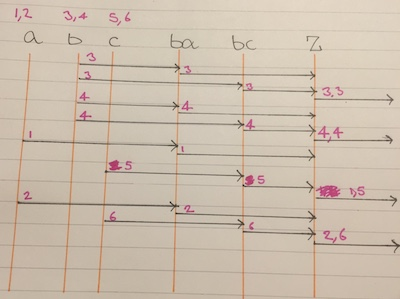
\includegraphics{figs/hand/append2zip-swim.jpg}
\caption[placeholder]{placeholder sequence diagram for an execution of @append2zip@.}
\label{figs/hand/append2zip-swim}
\end{figure}

The execution has two sections.
In the first section, all the values from the @b@ stream are pushed to both @append@ processes, then paired together.
In the second section, execution alternates between the other streams, @a@ and @c@, with one value from each.
The consumer process, @zip@, alternates between pulling from each of the @append@ processes.
The access pattern imposed by the consumer propagates upwards through the @append@ processes and to the input streams.

% \begin{lstlisting}
% (ba * bc) * z
% (bc * ba) * z
% (ba * z ) * bc
% (bc * z ) * ba
% (z  * ba) * bc
% (z  * bc) * ba
% ba * (bc * z )
% bc * (ba * z )
% ba * (z  * bc)
% bc * (z  * ba)
% z  * (ba * bc)
% z  * (bc * ba)
% \end{lstlisting}

This example contains three processes.
We could perform fusion in twelve different orders.
Of these twelve orders, there are two main categories.
The first category, we fuse the two @append@ processes together, then fuse with the @zip@ process.
In the second category, we fuse the @zip@ process with one of the @append@ processes, then fuse with the other @append@ process.

If we fuse the two @append@ processes together first, we interleave their instructions without considering the access pattern of the @zip@ process.
There are many ways to interleave the two processes; one possibility is that the fused process reads all of the shared prefix from stream @b@, then all of stream @a@, then all of stream @c@.
For the shared prefix, this interleaving alternates between pushing to streams @ba@ and @bc@.
After the shared prefix, this interleaving pushes the rest of the stream @ba@, then pushes the rest of the stream @bc@.
When we try to fuse the @zip@ process with the fused @append@ processes with this interleaving, we get stuck.
The @zip@ process needs to alternate between its inputs, which works for the shared prefix, but not for the remainder.
Fusing the two @append@ processes together caused us to prematurely commit to an interleaving that is locally correct for the two @append@ processes, but globally wrong.

Fusion succeeds in another order where we fuse the @zip@ process with one of the @append@ processes first, then fuse with the other @append@ process.
The consumer, @zip@, must dictate the order in which the @append@ processes push; fusing the @zip@ process first gives it this control.
We start from the consumer and fuse them upwards with their producers, because this allows the consumer to impose its access pattern on the producers.


\FigurePdf{figs/specconstr/append2zip}{Process network for append2zip}{Process network for append2zip}

To decide which order to fuse a whole network in, we treat the process network as a dependency graph.
\autoref{figs/specconstr/append2zip} shows the process network for @append2zip@, with producers at the top and consumers at the bottom.
The @zip@ depends on both @append@ processes, and each @append@ processes depends on its two input streams.
We find all the terminal processes, which are those consumers with no children processes that they produce to.
In our example, @zip@ is the only terminal process.

For each terminal process, we find its parents.
The terminal process in our example has multiple parents --- the two @append@ processes --- and we could fuse in either order.
In general, one parent may depend on another parent; in which case we first fuse with the parent which consumes from the other parent.
This allows the consuming parent to impose its access pattern upon the producing parent.
We repeatedly fuse each terminal process with its closest parent until there are no more parents.

After fusing each terminal process with all its ancestors, there may remain multiple processes.
This only occurs if the remaining processes do not share ancestors.
The remaining processes also cannot share descendents, since if they had descendents they would not be terminal.
This means the processes are completely separate and could be executed separately, in any order or even in parallel.
Having unconnected processes in the same process network is a degenerate case, as it could be represented as multiple process networks.
We err on the side of caution, telling the programmer about anything even slightly unexpected.
Rather than making the decision of which order to execute them in, we display a compile-time error and make the programmer separate the network.

The fusion algorithm for pairs of processes fails and does not produce a result process when two processes have conflicting access patterns on their shared inputs.
As the access patterns are determined statically, apparent conflicts may in fact never occur at runtime; we must approximate.
If at any point we encounter a pair of processes which we cannot fuse together, we display a compile-time error telling the programmer that the network cannot be fused.

\subsubsection{Future work}
\TODO{This likely belongs elsewhere}

This technique for determining fusion order is sound, because any order is sound.
Regardless of the order the processes are fused in, if fusion succeeds, the result process has the same meaning.

This fusion order works for the examples in \REFTODO{benchmarks}, but it is not complete.
Completeness for the fusion order means that if there exists any order in which fusion succeeds, then the order described above also succeeds.
% For large process networks, there are many orders we could fuse the processes.
% There are factorially many permutations of the set of processes, and on top of that, the fusion operation can be nested arbitrarily.
% This factorial number of possibilities is because the fusion algorithm is non-associative and non-commutative.
The order described above is a heuristic to avoid trying all possible orders, but it does not always work.

The following example, @append3@, is very similar to @append2zip@ except it returns three output streams constructed by appending the three input streams in different orders.

\begin{lstlisting}
append3 a b c =
  ab <- append a b
  ac <- append a c
  bc <- append b c
  return (ab, ac, bc)
\end{lstlisting}

This process network can be executed with no buffering.
First, read all of the @a@ input stream, then read the @b@ stream, then read the @c@ stream.
There is no single consumer in this example which imposes its access pattern on its producers, so our heuristic fails.
This process network can only be fused if the process that produces @ab@ and the process that produces @bc@ are first fused together.
If we fused @ab@ and @ac@ together first, the fusion algorithm would make an arbitrary decision of whether to read the @b@ stream before, after, or interleaved with the @c@ stream.
The heuristic described will not necessarily choose the right order.
Looking at the dependency graph alone, it is impossible to tell which is the right order for fusion.
If we replaced the @append@ processes with @zip@ processes, the dependency graph would remain the same, but either fusion order would work.

We propose to solve this in future work \REFTODO{future of fusion} by modifying the fusion algorithm to be commutative and associative.
These properties would allow us to apply fusion in any order, knowing that all orders produce the same result.

The fusion algorithm is not commutative because when two processes are trying to execute instructions which could occur in either order, the algorithm must choose only one instruction.
Fusion commits too early to a particular interleaving, when there are multiple interleavings that would work.
By explicitly introducing non-determinism in the fused process, we can represent all possible interleavings, and do not have to commit to one too early.
We are moving the non-determinism from the order in which fusion occurs, and reifying it in the process itself.

Reifying the non-determinism in the processes will mean that all fusion orders produce the same process at the end.
Different orders will not affect the result, or whether things fuse.
Different orders do affect the size of the intermediate process, before all processes are fused together.
Fusing two unrelated processes which read from different streams introduces a lot of non-determinism: at each step of the fused process, either of the original processes can take a step.
The two processes do not constrain each other and the result process will have a lot of states.
Fusing related processes, for example a producer and a consumer, introduce less non-determinism because there are points when only one of the processes can run.
When the consumer is waiting for a value, only the producer can run.
Generally, fusing related processes will produce a smaller process than fusing unrelated processes.
The size of the overall result for the entire network is not any different, but the intermediate process will be smaller.
Larger intermediate programs generally take longer to compile, so some heuristic order which fuses related processes is likely to be useful, even if the order does not affect the result.


% \subsection{Fusing a pair of processes}
% Fusing a pair of processes is slightly different because variables are passed as function arguments, instead of a global heap.
% It also needs to take into account variable bindings per label, because of the locally-bound variables.
% For a pair of labels, the variables is the union of variables in the original processes, as well as any \emph{new} channel buffers which need to be bound.
% These are the ones which have an input state of \emph{have}.

\subsection{Jump contraction}
Between fusing each pair of processes in a process network, we want to simplify the fused process a bit.
The fusion algorithm introduces some extra jump instructions in the fused process.
Jump instructions do not provide any computational expressiveness, and we can make the process smaller by removing the jump instructions.
Because the fusion algorithm is already quite complex and hard to prove correct, we remove the jump instructions in a separate step after fusion.
It is easier to write two simple transforms than one complex transform.

We call this transform that removes jump instructions \emph{jump contraction}.
We will look at a fused process in order to understand jump contraction.

In the following example, @map2@, we take an input stream and transform it twice in a pipeline.

\begin{lstlisting}
map2 = $$(fuse $ do
  a <- source [||sourceOfFile "in.txt"||]
  b <- map    [|| f ||] a
  c <- map    [|| g ||] b
  sink c      [||sinkToFile  "out.txt"||])
\end{lstlisting}

This translates into the following process network with two processes; one for each @map@.

\begin{lstlisting}[linebackgroundcolor={
  \hilineFst{8}
  \hilineFst{9}
  \hilineFst{10}
  \hilineFst{11}
  \hilineFst{12}
  \hilineSnd{17}
  \hilineSnd{18}
  \hilineSnd{19}
  \hilineSnd{20}
  \hilineSnd{21}
  }]
Process network:
  Sources: a = sourceOfFile "in.txt"
  Sinks:   c = sinkToFile  "out.txt"
  Processes:
    Process "map f a":
      Inputs:  a; Outputs: b; Initial: b0
      Instructions:
        b0   = Pull  a b1 b3
        b1 e = Push  b (f e) b2
        b2   = Drop  a b0
        b3   = Close b b4        
        b4   = Done

    Process "map g b":
      Inputs:  b; Outputs: c; Initial: c0
      Instructions:
        c0   = Pull  b c1 c3      
        c1 e = Push  c (g e) c2     
        c2   = Drop  b c0
        c3   = Close c c4         
        c4   = Done
\end{lstlisting}

We fuse process (@map f a@) with process (@map f b@), to create a new process which pushes to outputs streams @b@ and @c@.
The instructions of each input process are highlighted differently; the same highlighting is used in the fused process to illustrate which input process each instruction comes from.
Each instruction in the fused process has a comment to the right describing the original process labels and the channel states.

\begin{lstlisting}[linebackgroundcolor={
  \hilineFst{8}
  \hilineCom{9}
  \hilineFst{10}
  \hilineSnd{11}
  \hilineSnd{12}
  \hilineFst{13}
  \hilineSnd{14}
  \hilineFst{16}
  \hilineSnd{17}
  \hilineSnd{18}
  \hilineCom{19}
}]
Process network:
  Sources: a = sourceOfFile "in.txt"
  Sinks:   c = sinkToFile  "out.txt"
  Processes:
    Process "map f a / map g b"
      Inputs:  a                  Outputs: b c                Initial: l0
      Instructions:
        l0   = Pull  a    l1 l7               -- b0, \{\},       c0, \{\}
        l1 x = Jump      (l2 (f x))           -- b1, \{\},       c0, \{\}
        l2 y = Push  b y (l3 y)               -- b1, \{have b\}, c0, \{have b\}
        l3 y = Jump      (l4 y)               -- b2, \{\},       c0, \{have b\}
        l4 y = Push  c (g y) l5               -- b2, \{\},       c1, \{\}
        l5   = Drop  a    l6                  -- b2, \{\},       c2, \{\}
        l6   = Jump       l0                  -- b0, \{\},       c2, \{\}

        l7   = Close b    l8                  -- b3, \{\},       c0, \{closed b\}
        l8   = Jump       l9                  -- b4, \{\},       c3, \{closed b\}
        l9   = Close c    l10                 -- b4, \{\},       c3, \{closed b\}
        l10  = Done                           -- b4, \{\},       c4, \{closed b\}
\end{lstlisting}

The fused process (@map f a / map g b@) produces to both streams.
The instructions for labels @l0@ to @l6@ are the main loop for each element of the input stream; instructions for labels @l7@ to @l10@ apply once the input stream is finished.
For the most part the fused process simply alternates between the two input processes.
The only interesting part is labels @l1@ to @l3@, where the (@map f a@) process is trying to push to the stream @b@ while the (@map g b@) process is trying to pull from the same.
The (@map f a@) process applies the function @f@ to the current element and pushes this value to the stream.
The fused process also pushes the value to the stream, while keeping a copy to pass as a local variable to the other half of the fused process.
The jump instruction at label @l1@ applies the @f@ function and passes it as an argument so it can be used twice without having to be recomputed.

The fused process has eleven instructions, while the inputs each had five.
The fused process has gotten bigger, and the four jump instructions comprise most of the growth.
We would like to remove them.

Looking at the jump instruction at label @l8@, we see that the close instruction at label @l7@ continues to @l8@, then follows the jump instruction to @l9@.
We modify @l7@ to continue straight to @l9@ without the intermediate step, and remove the instruction at label @l8@ entirely.
We can perform the same simplification at the jump instruction for label @l6@ by searching for occurences and replacing them with the jump's destination, @l0@.

The jump instruction at label @l3@ is a bit more complicated because it is parameterised.

Minimise performs simple skip/jump contraction to remove superfluous states.
If label @l@ is @jump m[x=e]@, anywhere that jumps to @l@, we want to replace with a direct jump to @m[x=e]@.
This is complicated by the variable updates attached to each label.
A label @l[u]@, which in turn jumps to @l'[u']@, must in fact be replaced with @l'[u'[u]]@, because the substitutions for both variable updates must be applied.

However, blindly joining the substitutions can duplicate work.
If we have the following label update: (@l[x = expensive 2]@) where @expensive@ is some costly operation, and we also have @l'[a=x, b=x]@, we do not want to duplicate the call to @expensive@ as @l'[a = expensive 2, b = expensive 2]@.
As a conservative approach, we only apply minimisation when all substitutions are only simple variables.

One must also beware of infinite loops, as in the case of @l = jump l[u]@.
Now, when looking up the `next' label for @l@, we keep a set of labels already seen.
If we encounter the same label twice, it is time to stop unfolding the definition.

This transform also performs a simple form of dead code removal, by removing unreachable labels.


\subsection{Cull outputs}

When one process in the network pushes to an output channel but no other processes read from the channel, we can simplify the process network by removing the channel and all instructions that push to it.
This situation is unlikely to occur in the original process network; a programmer would not introduce a channel without using it.
This situation does happen often in the intermediate process network after some processes have been fused.

Even though the @b@ process is no longer used, the fusion algorithm leaves 
When there are multiple consumers reading from one producer and we fuse a consumer with the producer, the result process must keep producing for the sake of the other consumers.


\begin{lstlisting}
map3 a =
  (b,c) <- map'map f g a -- (pbc)
  d <- map h b -- (pd)
  return (c, d)
\end{lstlisting}

Now we fuse the fused process @pbc@ with the process @pd@, to create a new process named @pbcd@.
The fused process produces three output streams, @b@, @c@ and @d@.
The output stream @b@ is no longer used anywhere; it is not read by any other process or mentioned.
At this point, we can simplify the @pbcd@ process and remove the pushes to @b@.


\begin{lstlisting}
map3 a =
  (b,c,d) <- map'map'map f g h a -- (pbcd)
  return (c, d)
\end{lstlisting}

To remove the pushes to stream @b@, we can replace every instruction (@Push b v l'@) with (@Jump l'@).

In this case we were only able to remove the stream @b@ after fusing all processes together, but it is often possible to do it earlier.

\begin{lstlisting}
map3 a =
  b <- map f a
  c <- map g b
  d <- map h b
  return (c, d)
\end{lstlisting}


% \subsection{Insert dups}
% Let's pretend that the fusion process handles this case, as is the proof and paper version



% -----------------------------------------------------------------------------
% \section{Optimisation}
% \label{s:Optimisation}
% \TODO{Elsewhere.}
% 
% After we have fused two processes together, it may be possible to simplify the result before fusing in a third. Consider the result of fusing @group@ and @merge@ which we saw back in Figure~\ref{fig:Process:Fused}. At labels @F1@ and @F2@ are two consecutive @jump@ instructions.
% The update expressions attached to these instructions are also non-interfering, which means we can safely combine these instructions into a single @jump@.
% In general, we prefer to have @jump@ instructions from separate processes scheduled into consecutive groups, rather than spread out through the result code.
% The (PreferJump) clauses of Figure~\ref{fig:Fusion:Def:StepPair} implement a heuristic that causes jump instructions to be scheduled before all others, so they tend to end up in these groups.
% 
% Other @jump@ instructions like the one at @F5@ have no associated update expressions, and thus can be eliminated completely. Another simple optimization is to perform constant propagation, which in this case would allow us to eliminate the first @case@ instruction. 
% 
% Minimising the number of states in an intermediate process has the follow-on effect that the final fused result also has fewer states. Provided we do not change the order of instructions that require synchronization with other processes (@pull@, @push@ or @drop@), the fusibility of the overall process network will not be affected.
% 
% Another optimization is to notice that in some cases, when a heap variable is updated it is always assigned the value of another variable. In Fig.\ref{fig:Process:Fused}, the @v@ and @x1@ variables are only ever assigned the value of @b1@, and @b1@ itself is only ever loaded via a @pull@ instruction. Remember from \S\ref{s:Fusion:FusingPulls} that the variable @b1@ is the stream buffer variable. Values pulled from stream @sIn1@ are first stored in @b1@ before being copied to @v@ and @x1@. When the two processes to be fused share a common input stream, use of stream buffer variable allows one process to continue using the value that was last pulled from the stream, while the other moves onto the next one. 
% 

% When the two processes are able to accept the next variable from the stream at the same time, there is no need for the separate stream buffer variable. This is the case in Figure~\ref{fig:Process:Fused}, and we can perform a copy-propagation optimisation, replacing all occurrences of @v@ and @x1@ with the single variable @b1@. To increase the chance that we can perform copy-propagation, we need both processess to want to pull from the same stream at the same time. Moving the @drop@ instruction for a particular stream as late as possible prevents a @pull@ instruction from a second process being scheduled in too early.
% To increase the chance that we can perform this above copy-propagation, we need both processess to want to pull from the same stream at the same time. In the definition of a particular process, moving the @drop@ instruction for a particular stream as late as possible prevents a @pull@ instruction from a second process being scheduled in too early. In general, the @drop@ for a particlar stream should be placed just before a @pull@ from the same stream. 

\section{Drop everything}
\TODO{Elsewhere.}

The purpose of the @drop@ instructions is to keep two consumers more closely synchronised.
Coordinating drops between two consumers ensures that one consumer cannot start processing the next element until the other has finished processing the current element.
Drop instructions are not necessary for correctness, or even for ensuring boundedness of buffers.
Without drops, the result program is still correct, but one process can overtake another by one element.
Overtaking leads to larger processes because there end up being two copies of the processing code.

Suppose we have two consumer processes @P@ and @Q@, both pulling from the same channel @C@.
Both processes need to agree about when to pull from the channel.

\begin{lstlisting}
P = process
  P1: c <- pull C
  P2: push CP c
  P3: drop C
  P4: jump P1

Q = process
  Q1: c <- pull C
  Q2: push CQ c
  Q3: drop C
  Q4: jump Q1
\end{lstlisting}

The processes @P@ and @Q@ both pull from @C@, then push to their own output channel, @CP@ and @CQ@ respectively, drop their input, then loop back to pull again.
If we execute @P@ and it pulls from @C@, it can keep executing and push to its output channel @CP@, then drop the input.
Now, @P@ has dropped its input, but cannot pull again yet.
There is no new value available to pull because the producer cannot push to @C@ yet, because @Q@ has not consumed its input.
The producer cannot push until @Q@ pulls and drops its input.
When @Q@ pulls from its input, the producer still cannot push until @Q@ drops its input.
Without drops, @P@ would be able to start processing the next element before @Q@ had finished the previous one.

By synchronising the two processes together, when we fuse we will only have one copy of the code that pulls each element.
Because @P@ can only start pulling again by the time @Q@ has dropped, this means @P@ and @Q@ must both be trying to pull at the same time, which means we can reuse the same instructions generated from the previous time they both pulled.
The example @PQ_drop@ shows the fused process with drop instructions.
Note that there is only one copy of each input process' code.
On the other hand, @PQ_no_drop@ shows the fused process without drop instructions.
In @PQ_no_drop@ there are two copies of pushing to @CP@, though the main loop only executes one per iteration: pushing the current element to @CP@, and the previous element to @CQ@.
As the processes get larger, and more processes are fused together, the issue of duplicating code becomes more serious.
There are two parts to this: first, we need to hold the entire process in memory to generate its code.
Secondly, as the generated assembly code gets larger, it is less likely to fit into the processor's cache.
Smaller code is generally better for performance.
Having two copies of the push to @CP@ means that any consumers of @CP@ must in turn have their code duplicated, with the pull instructions from @CP@ copied into both sites of the pushes.

\TODO{diagrams}
\begin{lstlisting}
PQ_drop = process
  P1Q1: c_buf <- pull C
        c_p    = c_buf
        c_q    = c_buf
        push CP c_p
        push CQ c_q
        drop C
        jump P1Q1

PQ_no_drop = process
  P1Q1:  c_buf <- pull C
         c_p    = c_buf
         c_q    = c_buf
         push CP c_p
  P2Q2:  c_buf <- pull c
         c_p    = c_buf
         push CP c_p
         push CQ c_q
         c_q    = c_buf
         jump P2Q2
\end{lstlisting}


\section{Related work}
Meta-Repa \cite{ankner2013edsl} also uses Template Haskell for code generation, and provides a similar distinction between typed interface and untyped code generation.
It provides a generalised abstract datatype (GADT) for its typed interface rather than using typed Template Haskell.
It was implemented before typed Template Haskell.

